\chapter{Introduction}\label{ch:introduction}
% \epigraph{Нації вмирають не від інфаркту. Спочатку їм відбирає мову.
% \\ 
% \textit{Nations don\textquotesingle t die from heart attacks. They go mute first.}}{Ліна Костенко \\ Lina Kostenko, Ukrainian poetess}

% \epigraphhead[10pt]{
% \epigraph{"evals are surprisingly often all you need"}{
% Greg Brockman, OpenAI President
% \footnote{\href{https://twitter.com/gdb/status/1733553161884127435}{Greg Brockman on X: "evals are surprisingly often all you need" / X}}
% }
% }

% The Ukrainian language is not at risk of dying, and as of 2023, this
% much is certain. But before 2014, the quote above was so incisive it
% \emph{hurt}.

The last 10 years have led to a resurgence of Ukrainian language,
especially its use in informal and non-academic contexts. This was
followed by an increase of resources dedicated to its study and use.

On a 2020 survey\cite{inclusion} on linguistic diversity in NLP, the
Ukrainian language was classed under "rising stars": languages with a
thriving community online but let down by insufficent labeled data.

This Thesis introduces the first Ukrainian-language LM benchmark, and as
part of it introduces a number of novel labeled datasets.

\begin{itemize}
\tightlist
\item
  \textbf{TODOs}:

  \begin{itemize}
  \tightlist
  \item
    think about the story I\textquotesingle m telling in the
    Introduction
  \item
    exactly how much Ukrainian history, linguistics and Bender and for
    what purpose
  \item
    In the context of Bender: emphasize how I created datasets
  \end{itemize}
\end{itemize}

\section{Historical context and bilingualism in the modern Ukrainian
language}\label{historical-context-and-bilingualism-in-the-modern-ukrainian-language}

\begin{quote}
\emph{L'Ukraine a toujours aspiré à être libre}\\
``Ukraine has always aspired to be free.'' \\ Voltaire, \href{https://books.google.com.ua/books?id=Lh8TAAAAQAAJ&pg=PA275&lpg=PA275&dq=\%22L\%E2\%80\%99Ukraine+a+toujours+aspir\%C3\%A9+\%C3\%A0+\%C3\%AAtre+libre\%22&source=bl&ots=gvCwzOT0nI&sig=ACfU3U2PCd60vC7uxL9hCteT47A0Iiq8og&hl=en&sa=X&ved=2ahUKEwjjuNuwqOb0AhUhpIsKHeHsCQcQ6AF6BAgUEAM\#v=onepage&q=\%22L\%E2\%80\%99Ukraine\%20a\%20toujours\%20aspir\%C3\%A9\%20\%C3\%A0\%20\%C3\%AAtre\%20libre\%22&f=false}{1731}\footnote{Voltaire, History of Charles XII, King of Sweden (1731)
~\cite{1817oeuvres}}
\end{quote}
% \footnote{\textbf{TODO}
%   format citation
%   \href{https://www.atlanticcouncil.org/blogs/ukrainealert/debunking-the-myth-of-a-divided-ukraine/}{Debunking
%   the myth of a divided Ukraine - Atlantic Council} citing
%   \href{https://books.google.com.ua/books?id=Lh8TAAAAQAAJ&pg=PA275&lpg=PA275&dq=\%22L\%E2\%80\%99Ukraine+a+toujours+aspir\%C3\%A9+\%C3\%A0+\%C3\%AAtre+libre\%22&source=bl&ots=gvCwzOT0nI&sig=ACfU3U2PCd60vC7uxL9hCteT47A0Iiq8og&hl=en&sa=X&ved=2ahUKEwjjuNuwqOb0AhUhpIsKHeHsCQcQ6AF6BAgUEAM\#v=onepage&q=\%22L\%E2\%80\%99Ukraine\%20a\%20toujours\%20aspir\%C3\%A9\%20\%C3\%A0\%20\%C3\%AAtre\%20libre\%22&f=false}{Oeuvres
%   complètes de Voltaire - Voltaire - Google Books}}

A significant number of people in Ukraine are bilingual (Ukrainian and
Russian languages), and most Ukrainians can understand both Russian and
Ukrainian \cite{kulyk2018shedding}.\\
The reasons for this include Ukraine\textquotesingle s geographical and
cultural proximity to Russia, as well as of consistent policy first of
the Russian empire and the Soviet Union.

This section sketches the history of the language, describes the
bilingual nature of Ukraine\textquotesingle s society and the impact of
historical state policies on its modern development.

The ongoing Russian invasion is viewed by many as a continuation of a
long-standing historical pattern, rather than an isolated incident. This
section doesn\textquotesingle t attempt to justify or challenge any
particular position regarding the events described, nor is meant to be a
definitive account, but I believe this perspective is important to
understanding the current linguistic landscape in Ukraine, as well as
the linguistic challenges and phenomena that had a direct relevance on
this thesis. 

\TODO{
(\textbf{TODO} mention how and which tasks are impacted by
this; sources for \textquotesingle many people believe\textquotesingle;
todo tie it with Ukrainians realizing stuff)

\begin{itemize}
\tightlist
\item
  todo: more synonyms for \textquotesingle policy\textquotesingle{}
\item
  todo: better title
\item
  todo: sources for everything-everything-everything
\item
  todo: I don\textquotesingle t need an h4 with one item --- move this
  one level up. Maybe mention Poland, then Russia everything.
\item
  sources

  \begin{itemize}
  \tightlist
  \item
    1987 book about the entire topic \cite{krawchenko1987social}
  \item
    Article
    \href{https://culture.pl/en/article/the-executed-renaissance-the-book-that-saved-ukrainian-literature-from-soviet-oblivion}{The
    Executed Renaissance: The Book that Saved Ukrainian Literature from
    Soviet Oblivion \textbar{} Article \textbar{} Culture.pl}
  \item
    Keeping a record is the best book on this
    \cite{1130282272476965120}
  \end{itemize}
\end{itemize}
}

\subsection{Intro (TODO better title)}\label{intro-todo-better-title}

The Ukrainian language belongs to the Slavic family of the Indo-European
languages (which also contains languages such as Polish, Czech, Serbian,
Bulgarian), specifically to the East Slavic branch, which contains
Belarusian, Russian, and Ukrainian~\cite{grenoble2010contact}. Towards
the end of the X century the East Slavonic group of diealects was
relatively uniform, with the differences separating Ukrainian, Russian
and Belarusian appearing since then, as the result of linguistic and
political processes. \cite{press2015ukrainian}

While all three are mutually intelligible to a certain extent, Ukrainian
has more in common with Belarusian than with Russian
\cite{press2015ukrainian}; outside the branch, Ukrainian has partial
intelligibility with Polish~\cite{rehbein2014check}.

This stems from the fact that in the 15th century, parts of what is now
Ukraine and Belarus were part of the Polish-Lithuanian commonwealth,
with Polish becoming the \emph{lingua franca} of Ukrainian-Belarusian
lands.

As a result, a large proportion of the Ukrainian lexicon consists of
borrowings from the Polish language, and vocabulary remains the
component of the language where the difference with Russian is most
immediately noticeable. \cite{press2015ukrainian}

\subsection{The suppression of Ukrainian in the Russian
Empire}\label{the-suppression-of-ukrainian-in-the-russian-empire}

In the Russian Empire, the broader imperial ideology sought to
assimilate various ethnicities into a single Russian identity (with
Russian as dominant language), and policies aimed at diminshing
Ukrainian national self-consciousness were a facet of
that.\cite{doi:10.1016/j.euras.2014.05.005}

Ukrainian (then officially called \emph{little Russian}
\cite{press2015ukrainian} and considered a dialect) was\footnote{the
  original source\cite{doi:10.1016/j.euras.2014.05.005} states that, to
  a certain extent, among many Russians and some Europeans --- still is.}
 stigmatized as a (uncultured
peasants\textquotesingle) dialect of Russian,
%, with its literature not taken seriously; 
the general attitude being that
"backward Ukrainians" needed to be "civilized" by Russia, by its
language and developed culture.\cite{doi:10.1016/j.euras.2014.05.005}

Attempts to extinguish a separate Ukrainian identity
weren\textquotesingle t limited by stigmatization --- the history of
Ukrainian language bans is long enough to merit a separate Wikipedia
page with the list, \footnote{\href{https://en.wikipedia.org/wiki/Chronology_of_Ukrainian_language_suppression}{Chronology
  of Ukrainian language suppression - Wikipedia}}
  with the more notable ones
in the Russian Empire being the 1863 \textbf{Valuev Circular}
(forbidding the use of Ukrainian in religious and educational printed
literature)\footnote{Also memorably stating that "a separate Little
  Russian language has never existed, does not exist and cannot exist,
  and that their dialect, used by commoners, is just the Russian
  Language, only corrupted by the influence of
  Poland"\cite{enwikisource:13111073}}\cite{dibrova2017valuev} and the \textbf{Ems
Ukaz}, a decree by Emperor Alexander II banning the use of the Ukrainian
language in print (except for reprinting old documents), forbidding the
import of Ukrainian publications and the staging of plays or lectures in
Ukrainian (1876)\cite{remy2017despite}.

\subsection{The convergence of Ukrainian and Russian in the Soviet
Union}\label{the-convergence-of-ukrainian-and-russian-in-the-soviet-union}

The first decade of Soviet Union brought \emph{Ukrainisation} as part of
a new Soviet nationalities policy, leading to a short-lived period of
flourishing for Ukrainian literature and culture in
general.\cite{5c48fce9-c05d-3d4e-94c1-cd6079bff660} In 1928, the first Ukrainian spelling reform attempted to create a single set of rules unifying the various dialects existing at the time.~\cite{karunyk2017ukrainian}

Many of the Ukrainian writers and intellectuals of that period became
what was later known as "the executed
Renaissance"\cite{1ad9e7d5-c0eb-33df-ae6c-1fdbd2549d75}:
% \footnote{A bio-bibliography published in 1984 attempts to quantify this, finding 236 writers "lost to Ukrainian literature" out of 1,087 writers active in 1928. "In terms of figures alone the losses were quite
  % significant, but in terms of literary quality and originality they
  % were devastating." \cite{1130282272476965120}} 
many of them were executed, incarcerated, exiled in the years to
follow\cite{1130282272476965120}, after the Soviet Union took a sharp
turn towards Russification in the late 1920s and in the multiple waves
of purges afterwards.
This included many of the members of the committee behind the 1928 spelling reform~\cite{karunyk2017ukrainian}.%, with the chairman committing suicide.

Then a new \textquotesingle spelling\textquotesingle{} reform was drafted
in 1933, without public discussion this time
\cite{5c48fce9-c05d-3d4e-94c1-cd6079bff660}. It had the stated goal of
removing alleged "burgeoise nationalist" and "pro-Polish" influences in
the previous one, especially by the withdrawal of "artificial barriers"
between the Ukrainian and Russian languages%
\footnote{Andrij Khvylia, the chairman of this commission, described the intent behind the reform in his 1933 book \textit{"Eradicate, Destroy the Roots of Ukrainian Nationalism on the Linguistic Front"}.   He was himself later repressed for nationalism, after \textit{his} reform was framed as an attempt to "tear Ukrainian culture away from the fraternal Russian culture". 

The state of Ukrainian linguistic institutions at that time — the author of the first 1928 reform committed suicide, no members of the Institute of the Ukrainian Scientific Language survived past 1933, it got replaced by the Institute of Linguistics, which was itself purged in 1937-1938 with the exception of two members — meant that no linguists remained to revise Khvylia's spelling.~\cite{5c48fce9-c05d-3d4e-94c1-cd6079bff660}
}\cite{karunyk2017ukrainian}.
In practice, bringing the Ukrainian language closer to Russian in many
ways, from banning the (absent in Russian) letter \emph{ґ} to
introducing changes to grammatical forms \cite{karunyk2017ukrainian},
adding near absolute reliance on Russian when spelling loanwords and
changing the gender of many of them to match Russian, and by making an
effort to reduce Ukrainian-specific
vocabulary\cite{5c48fce9-c05d-3d4e-94c1-cd6079bff660}, especially
scientific terminology.

The role of Russian in Soviet society was openly declared to be not just
the language of all Soviet peoples, but also the source language for the
enrichment of the other languages in the Soviet
Union.\cite{press2015ukrainian}

\TODO{
\textbf{TODO} find some place to fit this:
One interesting aspect is the asymmetry in language intelligibility:
Ukrainians are "clearly more successful" in understanding Russians
than vice versa \cite{rehbein2014check}. If this mutual
understanding was only the result of the closeness of the two
languages, there would be no such asymmetry.
}

Towards the end of the Soviet Era, "it is possible to speak of diglossia
in Ukraine, with Russian as the High variety used in formal,
administrative, and educational domains, and Ukrainian is less formal,
home settings." \cite{grenoble2010contact}

After the fall of the Soviet Union, there were many proposals for
restoring the original orthography, but only the letter \emph{ґ} was
restored. In 2019 a new version of the Ukrainian orthography was
approved, which restored some of the original rules as
\textquotesingle legal\textquotesingle{} variants but without mandating
any of them.

\subsection{The contemporary Ukrainian linguistic
landscape}\label{the-contemporary-ukrainian-linguistic-landscape}

Around 2012, I stumbled upon a forum thread with the topic
"I\textquotesingle m moving to Ukraine, which language should I learn,
Ukrainian or Russian?". One answer was "It doesn\textquotesingle t
really matter, and if someone will care too much about which language
you speak, they are not the people you want to speak to anyway" --- not
an uncommon sentiment at the time.

For most Ukrainians, the language spoken was/is \textbf{just not part of
one\textquotesingle s self-identification as Ukrainian}. Among those
surveyed across Ukraine in 2012-2017, only 2.7-4.9\% considered the
language spoken what determines their nationality (among those who
considered themselves Ukrainian it was 1.8-2.5\%, Russian ---
8.8-15.9\%) \cite{kulyk2018shedding}.

It is typical to speak e.g. Russian at school and Ukrainian at home
\cite{Racek2024}, or different languages with different family members
(for example, my entire life I spoke Ukrainian with my father and
Russian with my mother).

Conversations where different people use Russian or Ukrainian (without
any effort awkwardness or negative effects) were (and are) normal as
well. This is illustrated by a 2017 survey\cite{Matveyeva2017} of 2,007
respondents across Ukraine. It found that in the presence of a Ukrainian
speaker, 17\% of people will speak Russian and \textasciitilde18\% both
Russian and Ukrainian (in the other case, \textasciitilde29\% will speak
Ukrainian and \textasciitilde23\% both Russian and Ukrainian).

Just as typical is \emph{code-switching} --- changing the language or
dialect spoken within the same conversation, sometimes within the same
sentence \cite{Kanishcheva2023}. The Parliamentary Code-Switching
Corpus paper\cite{Kanishcheva2023} shows examples of this happening for
different reasons, such as: inserting quotes/idioms in Russian, using
Ukrainian legalese/cliches or law names, switching the language for
stylistic purposes (e.g. distinguishing between the official
\emph{Ukrainian} position and a personal one), triggered code-switching
(switching the language after using a word or name in the other
language), inserting individual words in the other language or just
heavily mixing both without clear motivation.

The latter is related to \emph{Surzhyk}, mixed Russian-Ukrainian speech
(variously defined as "a hybrid language that involves Russian and
Ukrainian in its creation"\cite{Sira2019} or "a pejorative collective
label for non-standard language
varieties"\cite{bernsand2001surzhyk}), widely spoken (and
more rarely written) across Ukraine, especially its eastern, southern
and central parts\cite{Sira2019}.

The Russian attack on Crimea in 2014 for many led to stronger attachment
to Ukraine and alienation from Russia, with surveys between 2012 and
2017 showing "a consistent and substantial shift"\cite{Racek2024} from
Russian linguistic and ethnic identification towards
Ukrainian\cite{kulyk2018shedding}, and the full-scale invasion of 2022
accellerated this process, as seen in Rating Group\textquotesingle s
March 2022 "Language Issue in Ukraine"
survey\cite{ratinggroupSixthNational}.

This was also quantified by an analysis \cite{Racek2024} of Ukrainian
Twitter data between 13th January 2020 and 10th October 2022, reporting
behavioural language changes across Russian-Ukrainian-English while
controlling for user turnover (users joining or leaving Twitter).

The plot (adapted from Figure 4 of \cite{Racek2024}) in Fig.~\ref{fig:twitter} shows an increase of the use of Ukrainian over Russian
(purple) starting before the full-scale invasion and sharply increasing
afterwards. 

\begin{figure}[t]
\centering
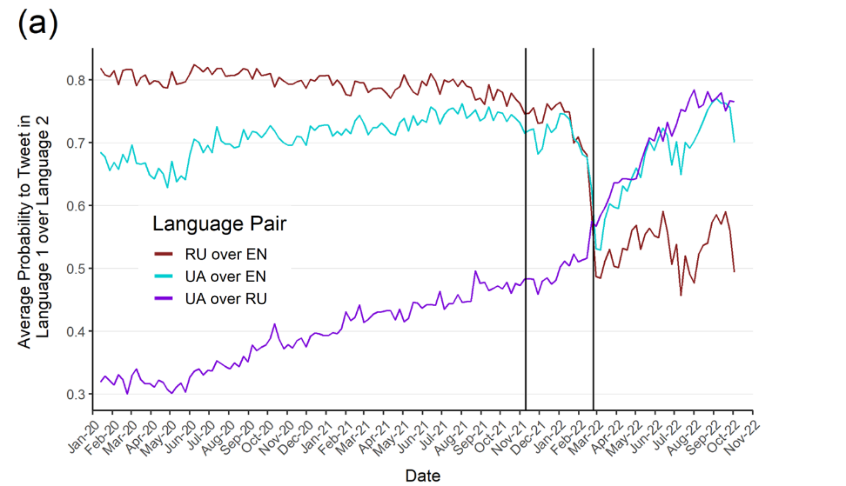
\includegraphics[width=1.0\linewidth]{Figures/ru_ua_twitter.png}
\decoRule
\caption[Ukrainian language dynamics on Twitter]{Tweeting language dynamics in 2020-2022; note the increase of the use of Ukrainian vs Russian (purple) throughout the period.}
\label{fig:twitter}
\end{figure}

Notably, of the 1,363 users tweeting predominantly (\textgreater80\%) in
Russian before the outbreak of the war, 61\% tweeted in Ukrainian more
after the outbreak, and \textasciitilde25\% (341) started tweeting
\emph{predominantly} (\textgreater80\%) in Ukrainian (hard-switch from
Russian to Ukrainian). There were only 3\% hard-switches from UA to RU
in that period.

Ukrainian Twitter users are not a representative sample of the Ukrainian
population for several reasons, but the study is likely indicative of
wider societal trends.

The authors interpret the switch as users\textquotesingle{} conscious
choice towards a more Ukrainian identity.\footnote{Switching from
  Russian to Ukrainian, for a habitual Russian speaker who considers Russian their mother tongue, is \emph{hard}.
  \href{https://newlinesmag.com/first-person/mother-tongue-the-story-of-a-ukrainian-language-convert/}{Mother
  Tongue: The Story of a Ukrainian Language Convert - New Lines
  Magazine}\cite{newlinesmagMotherTongue} tackles the emotional side of this for the many people who do make the effort.}

\TODO{
\textbf{TODO} fit the below somewhere:
\begin{itemize}
\tightlist
\item
  Many Ukrainians started critically reevaluating their language use
  patterns. (For example, I learned that two friends spoke Ukrainian at
  home but Russian at school not because they \emph{spoke Russian}, but
  because of (basically) peer pressure.)
\item
  mention the diglossia towards the end of USSR
\end{itemize}
}

With more people switching to Ukrainian partially or full-time, for
different reasons, the importance of Ukrainian NLP grows
correspondingly.

\section{Ukrainian as a mid-resource
language?}\label{ukrainian-as-a-mid-resource-language}

In the taxomy of languages based on data availability \cite{inclusion}
(see below), Ukrainian is classified in class 3, "the rising stars":
languages with a thriving online cultural community that got an energy
boost from unsupervised pre-training, but let down by insufficient
efforts in \emph{labeled} data collection. Sample languages from that
group include Indonesian, Cebuano, Afrikaans, Hebrew. (Russian is in
class 4, English and German are in class 5.)


\begin{figure}[t]
\centering
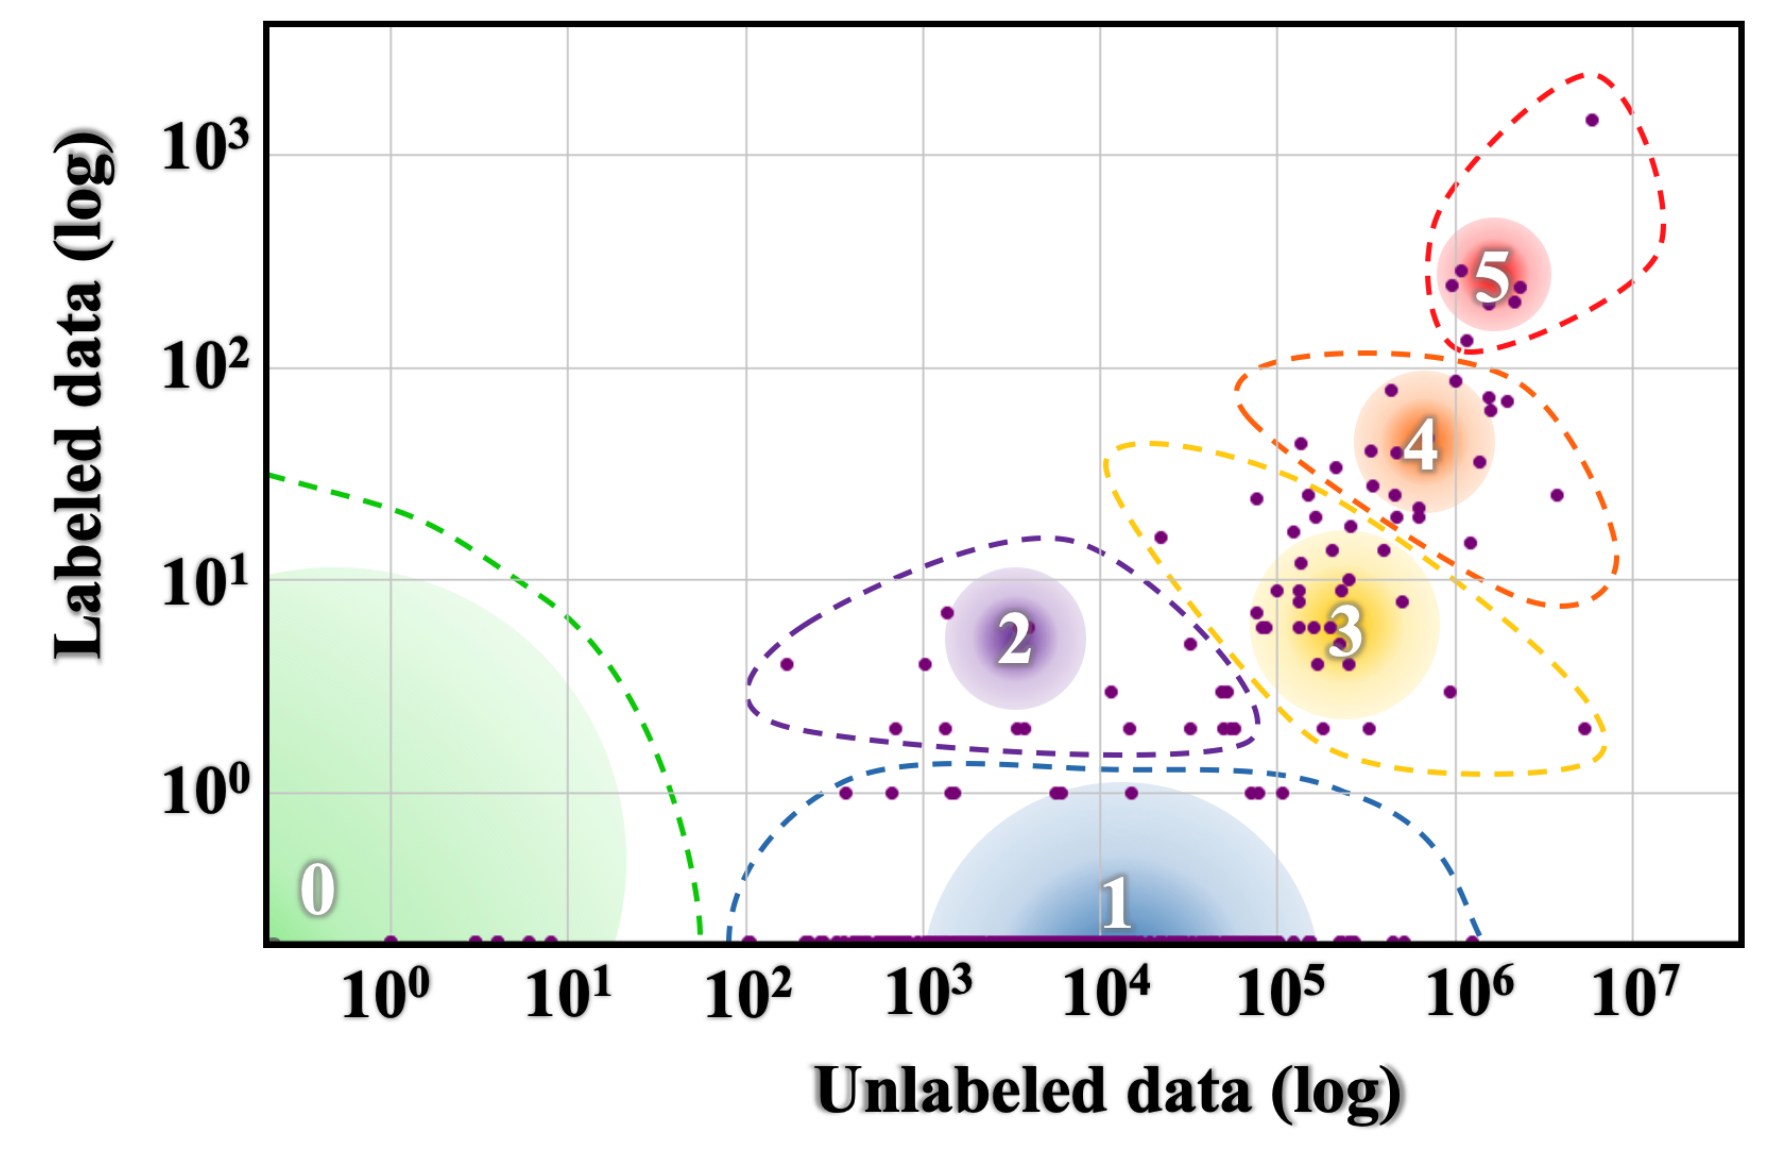
\includegraphics[width=1.0\linewidth]{Figures/Pasted image 20231030165827.png}
\decoRule
\caption[Language resource distribution]{Figure 2 of \cite{inclusion}, showing the language resource distribution. The size of the circle shows the number of languages in that class, the dashed lines show the points covered by that class. Ukrainian belongs to class 3.
% as quoted in \href{https://www.ruder.io/nlp-beyond-english/}{Why You Should Do NLP Beyond English}
}
\label{fig:bender}
\end{figure}

From a different angle, looking at estimates of languages used on the
Internet (as estimated percentages of the top 10M websites), as of
October 2023 Ukrainian is at number 19 (0.6\%), between Arabic and
Greek\cite{enwiki:1182341232}\footnote{quoting
  \href{https://w3techs.com/technologies/overview/content_language}{Usage
  Statistics and Market Share of Content Languages for Websites,
  September 2023} \cite{wiki:xxx}: \textless\_(@wiki:xxx) "List of
  Wikipedias/Table2 --- Meta, discussion about wikimedia projects"
  (2022) / Meta: \href{zotero://select/items/@wiki:xxx}{z} /
  \href{https://meta.wikimedia.org/w/index.php?title=List_of_Wikipedias/Table2&oldid=23936182}{\url{https://meta.wikimedia.org/w/index.php?title=List_of_Wikipedias/Table2&oldid=23936182}}
  / \emph{\textgreater{} \cite{Kanishcheva2023}:
  \textless{}}(@Kanishcheva2023) "The Parliamentary Code-Switching
  Corpus: Bilingualism in the Ukrainian Parliament in the 1990s-2020s"
  (2023) / Olha Kanishcheva, Tetiana Kovalova, Maria Shvedova, Ruprecht
  Von Waldenfels: \href{zotero://select/items/@Kanishcheva2023}{z} /
  \href{https://aclanthology.org/2023.unlp-1.10}{\url{https://aclanthology.org/2023.unlp-1.10}}
  / 10.18653/v1/2023.unlp-1.10 \_\textgreater{}}. English is \#1
(53.0\%), Russian \#3 (4.6\%), German at \#4 (4.6\% as well).

Ukrainian Wikipedia is 15th by daily views and by number of
articles\cite{wiki:xxx}.

\section{The importance of NLP for mid- and low-resource
languages}\label{the-importance-of-nlp-for-mid--and-low-resource-languages}

\subsection{The Bender rule and language
independence}\label{the-bender-rule-and-language-independence}

Emily M. Bender in 2011\cite{bender} formulated what would come to be
known as the Bender rule\cite{benderpost}: "Name the languages we
study".

Her original 2011 paper --- written in the pre-LLM era --- discusses the
problem of language independence, that is the extent to which NLP
research/technology can scale over multiple (or
\textquotesingle all\textquotesingle) languages. In her more recent
writing on the topic, she notes how work on languages other than English
is often considered "language specific" and thus viewed as less
important \cite{benderpost}, and the underlying misconception that
English is a sufficiently representative language and therefore work on
English is not language specific.

A NLP system that works for English is not guaranteed to behave
similarly for other languages, unless explicitly designed and tested for
that. Or in different words, \textbf{"English is Neither Synonymous with
Nor Representative of Natural Language"}. \cite{benderpost}

She highlights 8 proprieties of English that highlight
it\textquotesingle s shortcomings in representing all languages, of them
4 apply to Ukrainian: little inflectional morphology, fixed word order,
possible matches to database field names or ontology entries, and
massive amounts of training data available.

In the context of this thesis, an interesting facet of this issue was my
intuitive assumption that Python\textquotesingle s \texttt{sort()} would
sort the letters in their alphabetical order --- which is what it does
in English --- which, for Ukrainian, it didn\textquotesingle t. In
hindsight absolutely unsurprising, but I find it absolutely fascinating
that for many English-only-speakers many things \emph{just work}, like
python\textquotesingle s \texttt{sort()} doing the intuitively correct
thing, and this is taken for granted (along with the assumption that it
works for other languages just as well, and that results and approaches
generalize). Having for the first time sorted Ukrainian letters in
Python I realize how all-encompassing such world models can be. (For
details about the sorting issue, see subsection \textbf{XXX} about the
LMentry-static-UA task.)

(\textbf{TODO} what do I want to say here exactly?)

\begin{itemize}
\tightlist
\item
  Ukr. datasets on the HF Hub being in Russian
\item
  Random list of words contains Russian ones:
  \href{https://raw.githubusercontent.com/hermitdave/FrequencyWords/master/content/2016/uk/uk_50k.txt}{\url{https://raw.githubusercontent.com/hermitdave/FrequencyWords/master/content/2016/uk/uk_50k.txt}}
\item
  labs.perplexity.ai models \textbf{answering in Russian when asked for
  a Ukrainian folk tale} (see Tagebuch for 22-01-2024: {[}{[}231010-1003
  Masterarbeit Tagebuch\#\^{}90748a{]}{]})
\end{itemize}

\section{Roadmap}\label{roadmap}

This master thesis tackles the following problems in the context of
Ukrainian language:

\begin{itemize}
\tightlist
\item
  Research the current state of NLP, especially focusing on the
  availability and quality of:

  \begin{itemize}
  \tightlist
  \item
    datasets
  \item
    corpora
  \item
    tools
  \item
    literature
  \end{itemize}
\item
  Create novel Ukrainian-language datasets usable as benchmark tasks:

  \begin{itemize}
  \tightlist
  \item
    create human baselines where practicable
  \item
    make them publicly available through established platforms
  \end{itemize}
\item
  Create a benchmark for the evaluation of LMs, using both the
  newly-created datasets/tasks and pre-existing ones
\item
  Evaluate the existing Ukrainian LMs on this benchmark
\end{itemize}

Additional research questions are:

\begin{itemize}
\tightlist
\item
  Evaluate whether cross/multi language models that include Ukrainian
  perform equally well to Ukrainian monolingual models
\item
  Research whether there\textquotesingle s a significant difference in
  scores of tasks translated to Ukrainian using automated methods as
  opposed to human translations
\item
  Compare the extent to which the language matters when solving
  problems, with the following languages:

  \begin{itemize}
  \tightlist
  \item
    Ukrainian
  \item
    English (high resource language)
  \item
    Russian (high resource language from the same language family as
    Ukrainian)
  \end{itemize}
\end{itemize}

\chapter{Theory}\label{theory}

\section{Neural networks and stuff}\label{neural-networks-and-stuff}

\subsection{NLP and language modeling}\label{nlp-and-language-modeling}

\subsubsection{LMs}\label{lms}

\paragraph{Transformer-based}\label{transformer-based}

\paragraph{LLMs and their magic}\label{llms-and-their-magic}

\section{LM Evaluation}\label{lm-evaluation}

\subsection{Intrinsic/extrinsic eval}\label{intrinsicextrinsic-eval}

\begin{itemize}
\tightlist
\item
  Definition and examples
\end{itemize}

\subsubsection{Intrinsic}\label{intrinsic}

\begin{itemize}
\tightlist
\item
  Definition
\item
  Examples
\item
  Metrics (Perplexity, bpX etc.)
\end{itemize}

\subsubsection{Extrinsic}\label{extrinsic}

\begin{itemize}
\tightlist
\item
  Definition
\item
  Examples
\item
  Metrics
\end{itemize}

\subsubsection{Correlations between them and
interplay}\label{correlations-between-them-and-interplay}

\subsection{Zero/one/few-shot bits}\label{zeroonefew-shot-bits}

\section{LM benchmarking}\label{lm-benchmarking}

\subsection{Terminology}\label{terminology}

\begin{itemize}
\tightlist
\item
  from my first paper - task / dataset / benchmark / ...
\end{itemize}

\subsection{Taxonomy of benchmark
tasks}\label{taxonomy-of-benchmark-tasks}

\begin{itemize}
\tightlist
\item
  By task type/goal

  \begin{itemize}
  \tightlist
  \item
    Include more exotic/interesting ones, e.g. truthfulQA\footnote{\href{https://github.com/sylinrl/TruthfulQA/blob/main/TruthfulQA.csv}{TruthfulQA/TruthfulQA.csv
      at main · sylinrl/TruthfulQA}}
  \end{itemize}
\item
  One/two/X shot?...
\end{itemize}

\subsection{Benchmark data
contamination}\label{benchmark-data-contamination}

\subsubsection{Canary GUID strings}\label{canary-guid-strings}

\begin{itemize}
\tightlist
\item
  My own benchmark tasks have a canary string
\item
  The three ones from ua-datasets don\textquotesingle t, and are too
  available online - they might have become part of some LLM training
  data
\item
  \href{https://www.alignment.org/canary/}{Evaluations Canary~---
  Alignment Research Center} + BIG benchG
\end{itemize}

\subsection{Notable benchmark tasks}\label{notable-benchmark-tasks}

\begin{itemize}
\tightlist
\item
  Focus on individual tasks as opposed to bigger things
\item
  The usual ones e.g. in (Super)GLUE
\item
  If other languages\textquotesingle{} versions exist - mention them
\item
  Definitely list the ones I\textquotesingle ll use as base
\end{itemize}

\subsubsection{Children\textquotesingle s book
test}\label{childrens-book-test}

\subsubsection{Other}\label{other}

\begin{itemize}
\tightlist
\item
  TruthfulQA
\item
  Fact completion
\end{itemize}

\subsection{Notable benchmarks}\label{notable-benchmarks}

\begin{itemize}
\tightlist
\item
  non-UA but multilingual are OK
\item
  general examples and what makes them cool/notable,
  abstract/high-level, no lists of tasks
\end{itemize}

\subsubsection{HELM!}\label{helm}

\subsubsection{LMentry}\label{lmentry}

\subsubsection{BIGBench}\label{bigbench}

\subsubsection{GLUE, SuperGLUE}\label{glue-superglue}

\subsection{Benchmark (tasks)
desiderata}\label{benchmark-tasks-desiderata}

\begin{itemize}
\tightlist
\item
  How to build a good benchmark (task) in general
\item
  What does Ukrainian NLP need?

  \begin{itemize}
  \tightlist
  \item
    Modern but not too modern language

    \begin{itemize}
    \tightlist
    \item
      e.g. not the 1 million word story
    \end{itemize}
  \item
    Findability

    \begin{itemize}
    \tightlist
    \item
      Github
    \end{itemize}
  \item
    Ease of use

    \begin{itemize}
    \tightlist
    \item
      Upload datasets to HF
    \end{itemize}
  \item
    Implementation:

    \begin{itemize}
    \item
      Inclusion to other big benchmarks
    \item
      Implementations for important eval harnesses
    \end{itemize}
  \end{itemize}
\end{itemize}

\subsection{Evaluation harnesses}\label{evaluation-harnesses}

\begin{itemize}
\tightlist
\item
  What and why
\item
  My list in {[}{[}230928-1735 Other LM Benchmarks
  notes\#\textquotesingle evaluation harness\textquotesingle es{]}{]}
\item
  I decided to use X, instead of writing my own, because
\end{itemize}

\section{Ukrainian language}\label{ukrainian-language}

\subsection{Grammatical notation and
abbreviations}\label{grammatical-notation-and-abbreviations}

\subsubsection{Glossing notation}\label{glossing-notation}

Throughout this section, a notation system loosely based on the Leipzig
Glossing Rules\cite{comrie2008leipzig} (LGR) for interlinear glossing
will be used in examples showcasing Ukrainian language phenomena and
translations to English and occasionally German.

Interlinear glosses will not be interlinear, but each gloss will be a
superscript to the word it refers to.

For each word, it will be formatted thus:

\begin{itemize}
\tightlist
\item
  The translation will be separated with the grammatical morphemes
  relating to it by hyphens (-)
\item
  The translation to English will be written in lower case
\item
  The grammatical morphemes will be upper-case abbreviations separated
  by dots (LGR rule 3).
\end{itemize}

Not all words of the example will be annotated, only the ones relevant
to the \textbf{example} being made. Words already in English will not be
translated.

Each translation will be provided on a separate line, with the language
marked as ISO 639-3 code: \texttt{eng} for English, \texttt{ukr} for
Ukrainian, \texttt{deu} for German, \texttt{rus} for Russian.

For example:

\begin{gloss}[Example]{testnameref}
eng: the man\textsuperscript{NOM.SG} saw\textsuperscript{PST} the
dog\textsuperscript{NOM.SG}\\
ukr: чоловік\textsuperscript{man-NOM.SG} побачив\textsuperscript{saw-PST.MASC.SG}
собакy\textsuperscript{dog-ACC.SG}
\end{gloss}
% \ref{ex:testnameref}

In the cases where glosses on morpheme level are needed, the (relevant)
segmentable morphemes in the word will be separated by hyphens, and each
will have its gloss in its superscript\footnote{Unless a segmentation is
  needed only to have an adjacent morpheme that \emph{does} need a gloss
  segmented correctly --- then such a morpheme may not have a gloss.}.
The absence of a morpheme needing a corresponding gloss will be marked
as \(\varnothing\) (LGR Rule 6).

% \begin{quote}
\begin{gloss}{}
ukr: 5 собак\textsuperscript{dog}-\(\varnothing\)\textsuperscript{GEN.PL}
% \end{quote}
\end{gloss}

\textbf{Ungrammaticality} (examples of grammatically incorrect language)
will be denoted by a single asterisk (*) preceding the sentence or the
specific word:

\begin{gloss}{}
ukr: мій *друзь
\end{gloss}{}

\subsubsection{Abbreviations}\label{abbreviations-1}

These abbreviations are used inside glosses. They are mostly
conventional LGR abbreviations\footnote{See
  \href{https://en.wikipedia.org/wiki/List_of_glossing_abbreviations}{List
  of glossing abbreviations - Wikipedia} for a full list.} but contain
non-LGR ones as well, given as a separate list.

\begin{itemize}
\tightlist
\item
  Cases

  \begin{itemize}
  \tightlist
  \item
    NOM: Nominative
  \item
    ACC: Accusative
  \item
    DAT: Dative
  \item
    LOC: Locative (\textquotesingle table\textquotesingle{} in
    \textquotesingle the cup in on the table\textquotesingle)
  \item
    VOC: Vocative (used when addressing something)
  \end{itemize}
\item
  Number:

  \begin{itemize}
  \tightlist
  \item
    SG: Singular
  \item
    PL: Plural
  \item
    3PL: third person plural (they), 2SG: second person singular (you),
    etc.
  \end{itemize}
\item
  Gender: M for masculine, F for feminine, N for neutral
\item
  Tenses:

  \begin{itemize}
  \tightlist
  \item
    PST: Past
  \item
    FUT: Future
  \end{itemize}
\item
  Other:

  \begin{itemize}
  \tightlist
  \item
    PASS: passive
  \item
    REFL: reflexive (deu: \textquotesingle sich
    verspäten\textquotesingle)
  \item
    INF: infinitive
  \item
    CARD, ORD: cardinal/ordinal numeral
  \end{itemize}
\item
  Verb aspects:

  \begin{itemize}
  \tightlist
  \item
    IPFV: Imperfective (incomplete / habitual actions)
  \item
    PFV\footnote{Not to be confused with PERF (perfect \textbf{tense}),
      not used in this Thesis.}: Perfective (completed actions or ones
    viewed as a single whole).
  \end{itemize}
\item
  Verb moods:

  \begin{itemize}
  \tightlist
  \item
    IMP: Imperative (\textbf{TODO} worth it for confusion with IPFV?)
  \end{itemize}
\item
  Articles:

  \begin{itemize}
  \tightlist
  \item
    DEF, INDEF: definite, indefinite (the/an; der/ein etc.)
  \end{itemize}
\item
  Abbreviations not part of conventional LGR\footnote{Sometimes used,
    but absent from LGR proper since they are not glosses for
    morphological values.

    \begin{quote}
    Authors also use placeholders for generic elements in schematicized
    parsing, such as may be used to illustrate morpheme or word order in
    a language. Examples include head or hd
    \textquotesingle head\textquotesingle; root or rt
    \textquotesingle root\textquotesingle; stem or st
    \textquotesingle stem\textquotesingle; pref, prfx or px
    \textquotesingle prefix\textquotesingle; suff, sufx or sx
    \textquotesingle suffix\textquotesingle; clit, cl or encl
    \textquotesingle(en)clitic\textquotesingle; prep
    \textquotesingle preposition\textquotesingle{} and pos or post
    \textquotesingle postposition\textquotesingle, png
    \textquotesingle person--number--gender element\textquotesingle{}
    and tam \textquotesingle tense--aspect--mood
    element\textquotesingle{} (also ng number--gender, pn
    person--number, ta tense--aspect, tame
    tense--aspect--mood--evidential) etc. These are not listed below as
    they are not glosses for morphological values.
    (\href{https://en.wikipedia.org/wiki/List_of_glossing_abbreviations}{List
    of glossing abbreviations - Wikipedia}) \textbf{TODO} remove this
    \end{quote}}:

  \begin{itemize}
  \tightlist
  \item
    Parts of speech:

    \begin{itemize}
    \tightlist
    \item
      ADJ: adjective
    \item
      PRON: pronoun
    \item
      VERB, NOUN: verb, noun
    \end{itemize}
  \item
    Morphemes

    \begin{itemize}
    \tightlist
    \item
      PREF: prefix
    \item
      STEM: stem
    \item
      SUFX: suffix
    \end{itemize}
  \end{itemize}
\end{itemize}

\subsection{Ukrainian from a linguistic
perspective}\label{ukrainian-from-a-linguistic-perspective}

\subsubsection{Alphabet}\label{alphabet}

\begin{itemize}
\tightlist
\item
  \textbf{TODO} remove this subsection and move the problems paragraph
  somewhere else.
\end{itemize}

The Ukrainian alphabet is written in Cyrillic and has 33 letters, in
writing the apostrophe and hyphen are also used. It differs from Russian
by the absence of the letters \emph{ё, ъ, ы} and \emph{э}, and the
presence of \emph{ґ, є, і,} and \emph{ї}.

This helps (but doesn\textquotesingle t completely solve the problem of)
differentiating the two languages, which is needed relatively often:
Russian-language fragments within otherwise Ukrainian text (e.g.
untranslated quotes in text intended for a bilingual audience) are a
typical problem, and one that needs to be solved when building reference
corpora or datasets.\cite{9648705}

\subsubsection{Grammar}\label{grammar}

\paragraph{Strong morphology}\label{strong-morphology}

Ukrainian is is a \emph{synthetic\footnote{as opposed to analytic
  languages; Wikipedia has cool bits in
  \href{https://en.wikipedia.org/wiki/Synthetic_language}{Synthetic
  language - Wikipedia} e.g. antidisestablishmentarianism} inflected
language}\footnote{also known as \emph{fusional
  language}:\href{https://en.wikipedia.org/wiki/Fusional_language}{Fusional
  language - Wikipedia}}, that is it can express different grammatical
categories (case, number, gender, ..) as part of word formation. In
other words, that information about grammatical categories tends to be
encoded \emph{inside the words themselves}.\footnote{Another way to say
  this is that synthetic languages are characterized by a higher
  morpheme-to-word ratio.}

(German, too, is a fusional language, but with a smaller degree of
inflection. English, on the other hand, largery abandoned the
inflectional case system\footnote{except for personal pronouns;
  \href{https://en.wikipedia.org/wiki/English_grammar}{English grammar -
  Wikipedia}} and is an \emph{analytic} language, conveying grammatical
information through word order and prepositions.)

Specifically, Ukrainian:

\begin{itemize}
\tightlist
\item
  nouns decline for the 7 cases\footnote{including the \emph{vocative}
    case, absent in Russian, used when adressing someone (e.g.
    собак\textsuperscript{dog}-а\textsuperscript{NOM} when addressed becomes
    собак\textsuperscript{dog}-o\textsuperscript{VOC})} and 2 numbers (singular,
  plural)
\item
  adjectives agree with nouns in gender, case, number
\item
  verbs

  \begin{itemize}
  \tightlist
  \item
    conjugate for tenses, voices, persons, numbers
  \item
    and in the past tense, they agree with gender as well
  \end{itemize}
\item
  has no articles.
\end{itemize}

\paragraph{Inflection for word order}\label{inflection-for-word-order}

The standard word order is Subject-Verb-Object (SVO), but the
inflectional paradigm allows free word order. In English the SVO word
order in "the man saw the dog" (vs "the dog saw the man") determines who
saw whom. In Ukrainian it\textquotesingle s the last letter of the
object (dog) that marks it as such.

\begin{quote}
eng: the man\textsuperscript{NOM.SG} saw the dog\textsuperscript{NOM.SG}\\
ukr: чоловік\textsuperscript{man-NOM.SG} побачив\textsuperscript{saw}
собакy\textsuperscript{dog-ACC.SG}
\end{quote}

This allows the ordering of the words can be used for additional
emphases or shades of meaning (similar to German).

A more extensive example:

\begin{quote}
eng: we found\textsuperscript{PST} a green\textsuperscript{ADJ} cup \textsuperscript{NOUN} on
the table \textsuperscript{ADJ}\\
ukr: ми\textsuperscript{we} знайшли \textsuperscript{found-PST.1PL} зелену
\textsuperscript{green-ADJ.F.SG.ACC} чашку \textsuperscript{cup-F.SG.ACC}
на\textsuperscript{on} столі \textsuperscript{table-M.SG.LOC}\\
deu: wir\textsuperscript{we} fanden\textsuperscript{found-PST.1PL}
eine\textsuperscript{a-INDEF.F.SG.ACC} grüne\textsuperscript{green-ADJ.F.SG.ACC}
Tasse\textsuperscript{cup-F.SG.ACC} auf\textsuperscript{on}
dem\textsuperscript{the-DEF.M.SG.DAT} Tisch\textsuperscript{table-M.SG.DAT}
\end{quote}

The amount of categories conveyed by the nouns is roughly similar to
German.

\paragraph{Inflection in verbs}\label{inflection-in-verbs}

Morphology in verbs works in a very similar way. Additionally, unlike
other Slavic languages, Ukrainian has an inflectional future tense
(formed by a suffix in the verb) in addition to the standard compound
future formed by using an auxiliary word \emph{бути} ("to be").
\footnote{As an added layer of complexity, word stress can also impact
  grammatical categories. - \textbf{TODO} emphasize if I actually do a
  homonym-like task} All this makes longer verbs quite common.

For example, the verb \_ви́користати\_\textsuperscript{use-INF.PFV} is in
perfective aspect, therefore it\textquotesingle s a completed action
("use up" or "utilize completely") or one seen as a whole even if not
completed ("Tomorrow I\textquotesingle ll use my cane to get the pencil
from under the bed")\footnote{nice explanation: \textbf{TODO}
  remove\href{https://en.wikipedia.org/wiki/Perfective_aspect}{Perfective
  aspect - Wikipedia} /
  \href{https://en.wikipedia.org/wiki/Imperfective_aspect}{Imperfective
  aspect - Wikipedia}}. It can be transformed into
\_використовуватимуться\_\textsuperscript{use-IPFV-FUT-3PL-REFL}\footnote{Or
  \texttt{Aspect=Imp\textbar{}Mood=Ind\textbar{}Number=Plur\textbar{}Person=3\textbar{}Tense=Fut\textbar{}VerbForm=Fin}
  in CoNLL-U FEATS format.}\footnote{\textbf{TODO} thank him for this
  word?
  \href{https://twitter.com/Brooms1989/status/1611278169532768260}{Daniel
  Broomfield �������� on X: "Найскладніші слова в українській мові для мене:
  використовуватимуться високопоставленими абищиця (Ніколи не пам'ятаю,
  де поставити наголос ��)" / X}} (3rd person plural
imperfect-reflexive-future) thus (in bold the changes):

\begin{itemize}
\tightlist
\item
  використ\textsuperscript{use-ROOT}-а\textsuperscript{PFV}-ти\textsuperscript{INF}: to use
  (e.g. my cane to get home tomorrow)
\item
  використ\textsuperscript{use-ROOT}-ов\textsuperscript{}-увa\textsuperscript{IPFV}-ти\textsuperscript{INF}:
  to use (e.g. my cane from time to time)
\item
  використ\textsuperscript{use-ROOT}-ов\textsuperscript{}-увa\textsuperscript{IPFV}-ти\textsuperscript{INF}-муть\textsuperscript{FUT.3PL}:
  "They \emph{will use} their canes".
\item
  використ\textsuperscript{use-ROOT}-ов\textsuperscript{}-увa\textsuperscript{IPFV}-ти\textsuperscript{INF}-муть\textsuperscript{FUT.3PL}-ся\textsuperscript{REFL}:

  \begin{itemize}
  \tightlist
  \item
    "The canes \emph{will be used} tomorrow" (passive)
  \item
    "The mice \emph{will use themselves} to attract the cat into a trap"
    (reflexive)
  \end{itemize}
\end{itemize}

Minimal equivalent sentences:

\begin{quote}
eng: they \textsuperscript{3PL} will\textsuperscript{FUT} be\textsuperscript{PASS}
used\textsuperscript{PST.PTCP}\\
deu: sie\textsuperscript{they} werden\textsuperscript{will-FUT.PL}
verwendet\textsuperscript{used-PST.PTCP} werden\textsuperscript{be-PASS}\\
ukr: вони\textsuperscript{they}
використовуватимуться\textsuperscript{use-IPFV-FUT-3PL-REFL}\\
rus: они\textsuperscript{they} будут\textsuperscript{be-FUT.3PL}
использоваться\textsuperscript{use-INF-FUT-REFL}
\end{quote}

\textbf{Todo} (This is not a contrived example,
\emph{використовуватимуться} is a natural word in everyday speech.)

\paragraph{Numerals; agreement of nouns with
numerals}\label{numerals-agreement-of-nouns-with-numerals}

Ukrainian \textbf{numerals} can be cardinal (one), ordinal (first) and
adverbial (once). They change to varying extent based on case,
number\footnote{Some nouns can be used only in plural, e.g. in
  \emph{одні окуляри} (one \emph{pair} of glasses) the numeral
  \emph{one} is plural!}, gender.

The inflection of nouns for (grammatical) number has two classes,
singular and plural. Old East Slavic (from which Ukrainian is descended)
had a third grammatical number, the \emph{dual}, since lost\footnote{Parts
  of it --- to history, other parts --- explicitly forbidden in the 1932
  grammar reform.}. Some of its traces are in the \textbf{agreement of
nouns and numerals} (1 dog, 4 sheep, ...).

A simplified\footnote{This is only a partial description of both nouns
  agreement and numerals declination.} breakdown follows.

Numerals ending with the following numbers \textbf{require nouns to}:

\begin{itemize}
\tightlist
\item
  1: agree in gender, number, case with the numeral
\item
  2, 3, 4: require some nouns to be in the nominative plural, some -
  nominative singular\footnote{Mostly for some nouns of male gender
    (\emph{два громадянина})}
\item
  5-9, 0, 11-19: require the noun to be in the genitive plural
\end{itemize}

In practice, this means that "4 dogs" and "5 dogs" have a different
plural form for "dog":

\begin{quote}
чотири\textsuperscript{four-NOM}
собак\textsuperscript{dogs}-и\textsuperscript{\textbf{NOM.PL}}\\
пʼять\textsuperscript{five-NOM}
собак\textsuperscript{dogs}-\(\varnothing\)\textsuperscript{\textbf{GEN.PL}}
\end{quote}

This also means that the numerals (that can be inflected themselves!)
have to agree with the noun as well, for example the numeral
\textquotesingle one\textquotesingle{} in \textquotesingle one
dog\textquotesingle{} differs based on case:

\begin{quote}
ukr: \textbf{один\textsuperscript{one-MASC.NOM.SG}}
собака\textsuperscript{dog-MASC.NOM.SG}\\
eng: \textbf{one} dog
\end{quote}

\begin{quote}
ukr: немає\textsuperscript{there\textquotesingle s no}
\textbf{одного\textsuperscript{one-GEN.MASC.SG}}
собаки\textsuperscript{dog-GEN.MASC.SG}\\
eng: \textbf{one} dog is missing
\end{quote}

Lastly, the same holds for larger numerals ("four million", "five
million") even if they don\textquotesingle t have to agree with any
nouns: "million" (thousand, billion, ..) acts as a noun and four/five
acts as a numeral, bringing agreement issues even to a stand-alone
cardinal number.

\begin{itemize}
\item
  \textbf{Todo}

  \begin{itemize}
  \tightlist
  \item
    other Numbers to make it clear one is not special
  \item
    explain why i can\textquotesingle t replace gen pl with other gen pl
    - чоловіки and exceptions
  \end{itemize}
\item
  \textbf{TODO}
\item
  excellent:
  \url{http://kulturamovy.univ.kiev.ua/KM/pdfs/Magazine13-16.pdf}
\item
  list:
  \href{https://ukr.ed-era.com/chislivnik/uzgodzennya_chislivnikiv_z_imennikami}{Узгодження
  числiвникiв з iменниками - Українська мова: від фонетики до
  морфології}
\item
  complex examples: \href{https://zno.if.ua/?p=3542}{Узгодження
  числівника з іменником -- Українська мова та література}
\end{itemize}

\paragraph{Implications for NLP}\label{implications-for-nlp}

All the above has direct implications for NLP, for example:

\begin{itemize}
\tightlist
\item
  The development of lemmatizers, morphological analyses, bag-of-words
  approaches for information retrieval\cite{bender}
\item
  In the area of grammatical error correction, systems developed with
  English in mind perform worse for morphologically rich languages.
  \cite{Syvokon2022}
\item
  Correctly understanding the word order for the tone/intent/emphasis on
  specific parts of the sentence, as opposed to the arguably more
  explicit way English conveys this
\item
  Tools written for Russian can be made to work for Ukrainian but this
  doesn\textquotesingle t happen automatically, \emph{because the
  vocabulary and grammar are different}. \textbf{TODO}
\item
  \textbf{TODO} add more and more recent ones
\end{itemize}

In the context of this Thesis, inflecting words correctly has been the
most challenging aspect:

\begin{itemize}
\tightlist
\item
  In the CBT task, replacement nouns had to be inflected correctly so
  that morphology could not be used to get the correct answer. One
  initial area of concern was agreement of nouns with numerals --- to
  put the noun in the correct form there could have been a need to track
  not just the grammatical number (singular/plural), but also the
  \emph{actual} number of entities. At the end, this was handled by just
  using the form of the target word, which had already the correct
  inflection, and then manually filtering the edge cases. -
  \textbf{TODO} edit this when I actually do this, I
  don\textquotesingle t think I\textquotesingle ll have to track
  enything at the end - gen-pl can replace gen-pl and complex cases can
  just be excluded from the list
\item
  In the LMentry-static-UA task, different templates that used numbers
  ("what is the third word in the sentence", "what is in the third
  position in the sentence", etc.) the numbers had to be correctly
  inflected by case and gender
  (слово/\textquotesingle word\textquotesingle{} is neutral,
  позиція/\textquotesingle position\textquotesingle{} is feminine) as
  well.
\item
  Morphological analyses (needed for later inflection) required
  disambiguation, since different morphologies or even different POS can
  be written identically (\textquotesingle три\textquotesingle{} could
  be a numeral three, or an imperative verb meaning
  \textquotesingle cancel it!\textquotesingle). A correct disambiguation
  is crucial for future inflection. This necessitated the creation of a
  separate python package then used by most of the written tasks.
\item
  An additional edge case in the CBT task was that certain words
  (\textquotesingle converb\textquotesingle{} or
  \textquotesingle adverbial participles\textquotesingle{} that share
  features of both verbs and participles, e.g.
  \emph{приготувавши}/\emph{готуючи} (\textquotesingle having
  prepared\textquotesingle{} / \textquotesingle while
  preparing\textquotesingle)), tagged by pymorphy2 as POS \texttt{GRND}(
  corresponding to the Russian/Ukrainian POS
  \emph{деепричастие}\footnote{\href{https://pymorphy2.readthedocs.io/en/stable/user/grammemes.html}{Обозначения
    для граммем (русский язык) --- Морфологический анализатор pymorphy2}}/\emph{дієприслівник})
  are encoded in Universal Dependencies as POS \texttt{VERB} with
  feature \texttt{VerbForm=Conv}\footnote{\href{https://universaldependencies.org/u/feat/VerbForm.html}{VerbForm}}
  to represent the same concept. And, therefore, are detected as such by
  spacy\textquotesingle s Morphology. This meant that what spacy detects
  as \texttt{VERB}s required an additional morphological filtering step
  to exclude what pymorphy2 would see as \texttt{GRND}, because
  pymorphy2 isn\textquotesingle t able to inflect between (from its
  perspective different POS) \texttt{GRND} and \texttt{VERB}.
\end{itemize}

For list of other typological features of the language, see its page on
the World Atlas of Language Studies\cite{wals}\footnote{\href{https://wals.info/languoid/lect/wals_code_ukr}{WALS
  Online - Language Ukrainian} \cite{wals}: \textless\_(@wals) "WALS
  Online (V2020.3)" (2013) / : \href{zotero://select/items/@wals}{z} /
  \href{}{} / 10.5281/zenodo.7385533 \emph{\textgreater{}
  \cite{9648705}: \textless{}}(@9648705) "Ukrainian text preprocessing
  in GRAC" (2021) / Vasyl Starko, Andriy Rysin, Maria Shvedova:
  \href{zotero://select/items/@9648705}{z} / \href{}{} /
  10.1109/CSIT52700.2021.9648705 \emph{\textgreater{}
  \cite{synchak2023feminine}: \textless{}}(@synchak2023feminine)
  "Feminine personal nouns in ukrainian: Dynamics in a corpus" (2023) /
  Vasyl Starkoand Olena Synchak:
  \href{zotero://select/items/@synchak2023feminine}{z} / \href{}{} /
  \_\textgreater{}}, as well as the excellent "UD for Ukrainian" page on
the Universal Dependencies website\footnote{\href{https://universaldependencies.org/uk/index.html}{Ukrainian
  UD}}.

\chapter{Related work}\label{related-work}

\begin{itemize}
\tightlist
\item
  \textbf{TODO} Everywhere "Ukrainian X" - \textgreater{} "X in the
  Ukrainian language"??
\item
  The three Ukrainian evals in openai evals!
  \href{https://github.com/openai/evals/tree/main/evals/registry/data}{evals/evals/registry/data
  at main · openai/evals}

  \begin{itemize}
  \tightlist
  \item
    GEC!
  \end{itemize}
\end{itemize}

\section{Ukrainian NLP}\label{ukrainian-nlp}

\subsection{State of the research \&
literature}\label{state-of-the-research--literature}

\begin{itemize}
\tightlist
\item
  \href{https://aclanthology.org/2023.unlp-1.2/}{Contextual Embeddings
  for Ukrainian: A Large Language Model Approach to Word Sense
  Disambiguation - ACL Anthology}

  \begin{itemize}
  \tightlist
  \item
    Auto-generating WSD tasks based on SUM dictionary
  \end{itemize}
\item
  The intro of the UA-GEC paper \cite{Syvokon2022} links cool papers
  about how LMs done with "english in mind" are suboptimal for
  morphologically rich languages
\item
  \textbf{\href{https://github.com/robinhad/kruk}{robinhad/kruk:
  Ukrainian instruction-tuned language models and datasets}}

  \begin{itemize}
  \tightlist
  \item
    and the datasets linked there!
  \end{itemize}
\end{itemize}

\subsection{pymorphy2}\label{pymorphy2}

\begin{itemize}
\tightlist
\item
  Morphology analyzer
\item
  Not perfect for UA.

  \begin{itemize}
  \tightlist
  \item
    no score because no corpus? \cite{Korobov2015}
  \item
    Кір. КІР
  \item
    also has issues with \texttt{цар}
  \end{itemize}
\item
  they want to be cited as \cite{Korobov}, but I like the arxiv
  citation a bit more \cite{Korobov2015}
\item
  pymorphy3 exits! not used yet

  \begin{itemize}
  \tightlist
  \item
    does it do probability?..
  \end{itemize}
\item
  faster than spacy
\end{itemize}

\subsection{Datasets}\label{datasets}

\begin{itemize}
\tightlist
\item
  Inclusion criteria: ones that one could conceivably make into a
  benchmark task

  \begin{itemize}
  \tightlist
  \item
    e.g. not Instructions finetuning
  \end{itemize}
\item
  \href{https://arxiv.org/abs/2103.16997}{{[}2103.16997{]} UA-GEC:
  Grammatical Error Correction and Fluency Corpus for the Ukrainian
  Language}\cite{Syvokon2022}
\item
  \href{https://aclanthology.org/2023.unlp-1.2/}{Contextual Embeddings
  for Ukrainian: A Large Language Model Approach to Word Sense
  Disambiguation - ACL
  Anthology}\cite{labaContextualEmbeddingsUkrainian2023}
\end{itemize}

\subsubsection{Ukrainian-only}\label{ukrainian-only}

\begin{itemize}
\tightlist
\item
  All \texttt{ua-datasets}

  \begin{itemize}
  \tightlist
  \item
    \href{https://github.com/fido-ai/ua-datasets/tree/main/ua_datasets/src/token_classification}{POS
    tagging}
  \item
    \href{https://github.com/fido-ai/ua-datasets/tree/main/ua_datasets/src/question_answering}{SQuAD}
  \item
    \href{https://github.com/fido-ai/ua-datasets/tree/main/ua_datasets/src/text_classification}{News
    classification}
  \end{itemize}
\item
  \href{https://huggingface.co/datasets/vkovenko/cross_domain_uk_reviews}{vkovenko/cross\_domain\_uk\_reviews
  · Datasets at Hugging Face}
\end{itemize}

\subsubsection{\texorpdfstring{Multi/cross/... datasets that
\emph{include}
UA}{Multi/cross/... datasets that include UA}}\label{multicross-datasets-that-include-ua}

\textbf{Explicitly mention if it\textquotesingle s google translate or
real people did it}

\begin{itemize}
\item
  \href{https://paperswithcode.com/dataset/belebele}{Belebele Dataset
  \textbar{} Papers With Code} is a " multiple-choice machine reading
  comprehension (MRC) dataset", 122 languages
\item
  \href{https://github.com/KGQA/QALD_9_plus}{KGQA/QALD\_9\_plus:
  QALD-9-Plus Dataset for Knowledge Graph Question Answering} - one of
  the 9 langs is Ukrainian! One could theoretically convert the entities
  into text
\item
  \href{https://github.com/daniel-furman/polyglot-or-not}{daniel-furman/polyglot-or-not:
  {[}arXiv pre-print{]} Are foundation language models multilingual
  knowledge bases?}
\item
  ... somewhere: why can\textquotesingle t one just google translate
  existing benchmarks and be done with it? precision, eval, etc.
\end{itemize}

\chapter{Eval-UA-tion Ukrainian eval
benchmark}\label{eval-ua-tion-ukrainian-eval-benchmark}

\section{Basic description}\label{basic-description}

The benchmark contains \textbf{2} main tasks:

\begin{itemize}
\tightlist
\item
  CBT-UA (containing \textbf{XXX} test instances), which involves
  fill-in-the-gaps questions based on children\textquotesingle s
  stories. Gaps can be of three types: named entities (defined as
  animate nouns e.g. \textquotesingle Whiskers\textquotesingle{} or
  \textquotesingle tailor\textquotesingle), common nouns (grain, home),
  and verbs. The goal is that some understanding of the story
  (characters\textquotesingle{} motivations, etc.) is needed to
  correctly decide e.g. \emph{which} character was banished from the
  forest for stealing, or whether he stole grain (owned by his friend)
  or chickens (owned by his enemy). The idea is based on the
  Children\textquotesingle s Book Test task AAAAtaskCBTBBBB but contains
  many differences from it, most stemming from Ukrainian morphology.
\item
  LMentry-static-UA, which itself is composed of \textbf{XXX} subtasks,
  some quite different from each other. They are based on tasks that are
  simple for humans but suprisingly complex for LMs, such as "which word
  is first in alphabetical order", "what is the fifth letter of the word
  \textquotesingle orange\textquotesingle", or "do all words from this
  list belong to the same category: happiness, sadness, anger, plumber".
  It\textquotesingle s based on the LMentry task \cite{bm_lmentry} but
  departs from it in many ways, form the different subtasks to the
  change of evaluation mechanism (the original task was scored
  exclusively by regexes, this task is a dataset with exact anwers,
  hence the \emph{static} part in the name).
\end{itemize}

The tasks and the datasets connected to them are uploaded to the
HuggingFace Hub, and EleutherAI lm-evaluation-harness (widely used in
literature) \textquotesingle tasks\textquotesingle{} are implemented for
each (though not included in the harness itself).

\textbf{TODO} mention how I fulfill the criteria laid out in:

\begin{itemize}
\tightlist
\item
  \href{https://github.com/openai/evals/blob/main/docs/build-eval.md\#criteria-for-contributing-an-eval}{OpenAI
  evals checklist}
\item
  the multilingual paper bits
\item
  any other similar bits I find
\end{itemize}

\section{Construction}\label{construction}

\begin{itemize}
\tightlist
\item
  CBT task story generation story
\end{itemize}

\section{Validation and Human
evaluation}\label{validation-and-human-evaluation}

\subsection{Validation of the training
instances}\label{validation-of-the-training-instances}

As a first step, spot-checks of various training instances of the
datasets were performed as sanity check.

\subsubsection{LMentry-static-UA}\label{lmentry-static-ua}

LMentry-static-UA contained exclusively algorithmically generated tasks
with little randomness involved, and there the validity of the training
instances was especially strongly dependent on the code that generated
it --- and after looking at enough examples of "what\textquotesingle s
the Nth word in this sentence", one could safely assume the rest were
likely to be correct as well. So only a limited subset was manually
checked.

The only issue found was wrong ground truth in the task about
alphabetical ordering: the canonical order of the Ukrainian alphabet is
different from what python\textquotesingle s sorting does (with the
Ukrainian-only letters \emph{і} \emph{ї} \emph{є} \emph{ґ} being sorted
at the very end instead of their usual place in the Ukrainian alphabet).
The relevant code was rewritten to force the correct expected ordering.
(Section \textbf{XXX}* has some reflections on the implications of this
in the context of the Bender rule.)

\subsubsection{CBT-UA}\label{cbt-ua}

For the CBT-UA task (which involved creating training instances based on
data gained through ML approaches), the filtering of the resulting
dataset was much more involved.

There were two rough classes of error sources: those caused by language
and those caused by logic.

All the failure modes and their numbers are described its subsection
\textbf{XXX}, but suffice to say occasional incorrect lemmatization and
POS detection by spacy, incorrect normalization and detection (and
therefore inflection) by pymorphy2, and the best-guess approach used in
the \texttt{pymorphy-spacy-disambiguation} package (written specifically
for this Thesis) created a large area of uncertainty.

On the logic side, there were the unavoidable errors stemming from the
task creation approach (despite reasonable safeguards being put in place
where practical), such as multiple possible answers, unknowable answers,
etc.

\begin{itemize}
\tightlist
\item
  cases where there was more than one correct answer, e.g.

  \begin{itemize}
  \tightlist
  \item
    if there\textquotesingle s a tailor-turle
  \item
    the turtle is a both a turtle and a tailor, and where a gap
    contained "turtle" using "tailor" there would be correct as well,
    and both options are included in possible answers:
  \item
    "the tailor-turtle started sewing/working": again, working would be
    a
  \end{itemize}
\end{itemize}

\section{Construction, validation, ...}\label{construction-validation-}

\begin{itemize}
\tightlist
\item
  truthfulQ\cite{linTruthfulQAMeasuringHow2022} paper has examples
\item
  \textbf{LOOK WHETHER MY BENCHMARK IS PART OF THE TRAINING DATA!!!} -
  doing interesting tests on the topic
\end{itemize}

\section{Benchmark tasks}\label{benchmark-tasks}

\subsection{POS tagging}\label{pos-tagging}

\href{https://github.com/fido-ai/ua-datasets/tree/main/ua_datasets/src/token_classification}{POS
tagging}

\subsection{UA-SQuAD}\label{ua-squad}

\href{https://github.com/fido-ai/ua-datasets/tree/main/ua_datasets/src/question_answering}{SQuAD}

\subsection{LMentry-static-UA}\label{lmentry-static-ua-1}

\begin{itemize}
\tightlist
\item
  {[}{[}231203-1745 Masterarbeit eval task LMentry-static-UA{]}{]} for
  the progress \textbf{TODO}
\end{itemize}

This dataset is a set of tasks loosely on the original LMentry
evaluation task\cite{bm_lmentry} described in section \textbf{XXX}.

\begin{itemize}
\tightlist
\item
  TODO note

  \begin{itemize}
  \tightlist
  \item
    tokenization within sentences (новобранців-іноземців, 100 000)

    \begin{itemize}
    \tightlist
    \item
      within words: пліч-о-пліч how many LETTERS? what about варʼят?
    \end{itemize}
  \end{itemize}
\end{itemize}

\subsubsection{Differences from LMentry}\label{differences-from-lmentry}

The original LMentry \cite{bm_lmentry} had a list of \textbf{20-XXX}
partly repetitive tasks, e.g. "bigger number" and "smaller number" being
separate ones.

LMentry-static-UA (in addition to applying the ideas to Ukrainian)
contains the following conceptual changes:

\begin{itemize}
\tightlist
\item
  Only \emph{static} tasks are included. The original benchmark uses
  regular expressions for evaluating the tasks in the included scripts,
  but regexes are (strictly speaking) needed only for the tasks of type
  "write word/sentence {[}(not) containing \textbar{} starting/ending
  with {]} the following word/letter". To simplify inclusion in other
  benchmarks, as well as to not require custom evaluation code, these
  tasks were dropped, and the LMentry-static-UA tasks can be distributed
  as-is in the form of datasets.
\item
  Tasks are grouped by type, e.g. task type \texttt{CompareTwoThings} is
  a parent type of \texttt{LetterCount} (containing both
  \textquotesingle more\textquotesingle{} and
  \textquotesingle less\textquotesingle{} letters) and
  \texttt{NumberComparison} (bigger+smaller) number. This was done to
  reduce repetitive code and to decrease the number of tasks to contain
  only conceptually different ones.
\item
  The tasks about first/last entities have been expanded to counting,
  e.g. in addition to "what is the last word in the sentence"
  there\textquotesingle s also "what is the \emph{fourth} letter in this
  sentence".
\item
  \textbf{TODO} not yet implemented but will be:

  \begin{itemize}
  \tightlist
  \item
    The task about comparing two numbers has been expanded to basic
    comparison tasks, e.g. "the red box contains two million pens and
    the blue box has five hundred thousand thirteen pens; which box has
    more pens?"
  \end{itemize}
\end{itemize}

\subsubsection{Dataset structure}\label{dataset-structure}

The LMentry-static-UA dataset is shared on Huggingface under the link
\textbf{XXX}. Since the individual tasks are different, multiple configs
are contained in the dataset, with e.g. the \texttt{NumberComparison}
subtask being available as \TODO{TODO}

\subsubsection{Dataset construction}\label{dataset-construction}

\begin{itemize}
\tightlist
\item
  Different templates for the same question
\item
  UUIDs to make analysis simpler
\item
  Metadata
\end{itemize}

\subsubsection{List of tasks included}\label{list-of-tasks-included}

\subsubsection{Human evaluation}\label{human-evaluation}

\subsubsection{Challenges in the
implementation}\label{challenges-in-the-implementation}

\paragraph{Agreement}\label{agreement}

As with other tasks, agreement of Ukrainian numerals and nouns (see
section \textbf{XXX}) has taken a large amount of time.

The different templates contained different nouns in the same role
(first word, word one, first position, etc.) that required cardinal and
ordinal numerals. They had to agree with the noun in gender (number as
well, but in practice only singular was needed \textbf{TODO}):

\begin{quote}
eng: The \emph{third} \emph{word} in the sentence is ...\\
ukr: Третє\textsuperscript{third-3SG.N.ORD} слово\textsuperscript{word-3SG.N} ...
\end{quote}

This raised two problems.

\paragraph{Encoding and formalization}\label{encoding-and-formalization}

When creating a template, where/how to encode whether this template
requires an ordinal/cardinal and agreed to which grammatical categories.

\textbf{SOLUTION}: \textbf{including capitalized numerals in the correct
form in the template itself} and automatically parsing the grammatical
categories needed from them:

\begin{quote}
eng: The FIRST\textsuperscript{ORD} word in the sentence is ...\\
eng: Word number ONE\textsuperscript{CARD} in the sentence is ...\\
ukr: ПЕРШЕ\textsuperscript{first-3SG.N.ORD} слово\textsuperscript{word-3SG.N} ...
\end{quote}

This allowed to create templates using natural language and simplified
the data structures involved.

\paragraph{Creation of the training instances with
agreemeent}\label{creation-of-the-training-instances-with-agreemeent}

When constructing the actual training instances from the templates:

\begin{enumerate}
\def\labelenumi{\arabic{enumi}.}
\tightlist
\item
  all capitalized words are morphologically analyzed with pymorphy2 to
  get the needed grammatical categories
\item
  the int number needed for the training instance is converted to either
  ordinal or cardinal numeral in the normal form (\texttt{NOM.M.SG})
\item
  the resulting numeral in inflected to match the capitalized word in
  the template
\end{enumerate}

The implementation of this was challenging, and resulted in the creation
of a separate pyhon package,
\href{https://github.com/pchr8/ukr_numbers/}{ukr\_numbers}, which
creates numerals based on an input integer and a natural language
description of the needed inflection:

\begin{minted}{python}
>>> from ukr_numbers import Numbers
>>> Numbers().convert_to_auto(15,"перший")
'пʼятнадцятий'

# loosely paraphrasing to English: 
>>> convert_to_auto(15, "first")
"fifteenth"
\end{minted}

Under the hood, it uses
\href{https://pypi.org/project/num2words/}{num2words} to generate
Ukrainian ordinals/cardinals in normal form and the already mentioned
\href{https://github.com/pymorphy2/}{pymorphy2} to parse the natural
language form and inflect the numeral.

The otherwise excellent \texttt{num2words} was not able to inflect
Ukrainian ordinals by case, necessitating manual pymorphy2 inflection
logic and leading to many edge cases:

\begin{itemize}
\tightlist
\item
  pymorphy2 can analyze and inflect only single words (Ukrainian
  numerals can contain multiple words)
\item
  disambiguating between different pymorphy2 analyses was complex

  \begin{itemize}
  \tightlist
  \item
    some cases were trivial, e.g. some words being parsed as both verbs
    and numerals (три\textsuperscript{three-NUM} /
    три\textsuperscript{cancel-2SG.IMP}) was not an issue because we know
    we\textquotesingle re dealing with numerals
  \item
    some harder but not an issue, e.g. some grammatical categories
    can\textquotesingle t be disambiguated from the word itself (e.g.
    перший\textsuperscript{first-ORD.M?/N?} can be masculine or neutral) but
    this doesn\textquotesingle t matter because after inflection they
    will be indistinguishable as well
  \item
    etc. \textbf{TODO}
  \end{itemize}
\item
  inflecting multiple-word numerals was a whole \textbf{bundle of joy}

  \begin{itemize}
  \tightlist
  \item
    ordinals ending in 10\^{}2 or 10\^{}3, 10\^{}6, 10\^{}9 .. are
    written together (3000 -\textgreater{} \emph{тритисячний}), others
    aren\textquotesingle t (3001-\textgreater{} \emph{три тисячі
    перший})
  \item
    in "one/four/five thousand/millions/...", million \textbf{acts as a
    noun}, \textbf{necessitating noun and numeral agreement}. And as
    mentioned in section \textbf{XXX}, nouns \textbf{take different
    forms based not on singular/plural, but the actual number involved}
    (plurals aren\textquotesingle t just plurals, 2-3-4 are different
    from 5+)

    \begin{itemize}
    \tightlist
    \item
      singular/plural conversions for Ukrainian in pymorphy2 was broken,
      along with the function \texttt{make\_agree\_with\_number} that
      depended on it, leading to a bug report\footnote{\href{https://github.com/pymorphy2/pymorphy2/issues/169}{Числа
        и проблемы с склонением в разборах всех украинских слов · Issue
        \#169 · pymorphy2/pymorphy2}} and cumbersome workaround from my
      side
    \end{itemize}
  \end{itemize}
\end{itemize}

Not all edge cases are solved, but in all cases relevant to the
LMentry-static-UA tasks it works as expected and produces grammatically
and semantically correct output.

\subsection{Children\textquotesingle s book test
(CBT)}\label{childrens-book-test-cbt}

\subsubsection{Basics}\label{basics}

\textbf{TODO} The following terms will be used throughout this section:

\begin{itemize}
\tightlist
\item
  A \textbf{story} is divided into two parts, the \textbf{context
  segment} (the first 65\% of the sentences) and the \textbf{challenge
  segment} (the last 35\%).
\item
  The challenge segment contains a \textbf{gap}: the place where a token
  is masked/removed (replaced with \texttt{\_\_\_\_\_}).
\item
  The taks is multiple-choice, with \textbf{options} being the 6 tokens
  provided as possible replacements, only one of them being the
  \textbf{correct answer}.
\item
  A single test instance (with a gap and corresponding options) is a
  \textbf{task instance}.
\end{itemize}

\subsubsection{A taxonomy of ways task instances can be
wrong}\label{a-taxonomy-of-ways-task-instances-can-be-wrong}

During manual task instance filtering, the task instances were
classified into usable and unusable, with the latter removed from the
dataset. There were different reasons an instance would be unusable.
These reasons were formalized into a simple taxonomy. This was
originally done for the people helping with the filtering, in the form
of annotation guidelines and with checkboxes in the labeling interface
serving chiefly as reminders of the problems to look for.

The errors can be divided into three different (albeit fuzzy) types:

\begin{enumerate}
\def\labelenumi{\arabic{enumi}.}
\tightlist
\item
  Logic/continuity errors:

  \begin{itemize}
  \tightlist
  \item
    \textbf{Cause}:

    \begin{itemize}
    \tightlist
    \item
      The way the tasks are created, which doesn\textquotesingle t take
      into accounts the fact that different words belonging to the
      classes of the gap may refer to the same entity
    \item
      The decision where to place gaps doesn\textquotesingle t take into
      account the story narrative (but only the location of the gap,
      frequency of the lemma, and availability of enough different
      options)
    \end{itemize}
  \item
    \textbf{Kinds}:

    \begin{enumerate}
    \def\labelenumii{\arabic{enumii}.}
    \tightlist
    \item
      Answer unknown - The story doesn\textquotesingle t contain
      information that allows the answer to be inferred. -
      \textgreater{} The Cat and the Turtle go to
      \textbf{Cat/Turtle/Lion}\textquotesingle s house to sew the coat,
      and later deliver it to the Lion\textquotesingle s house. - The
      house is mentioned only once and has no dependencies to the rest
      of the narrative. One can infer that it\textquotesingle s not the
      Lion\textquotesingle s house (since it\textquotesingle s clearly a
      different place they have to go to), but there\textquotesingle s
      no way to know if it was Cat\textquotesingle s or
      Turtle\textquotesingle s. - However, if the options were only
      "\textbf{Cat/Lion}\textquotesingle s house" this would be a valid,
      solvable instance. - Similarly, if the Cat lived in a castle, this
      would also be considered a solvable instance.
    \item
      Multiple options are correct

      \begin{itemize}
      \tightlist
      \item
        It\textquotesingle s clear what entity/action is involved, but
        there are multiple options which fit it.

        \begin{itemize}
        \item
          \begin{quote}
          The Lion liked the Cat and Turtle\textquotesingle s
          \textbf{coat/work}. Both \textbf{tailors/animals} were happy.
          \end{quote}
        \item
          \begin{quote}
          Whiskers was happy that he was a cat: he was fast and could
          climb trees. One morning, he heard his owner say: "Our
          \textbf{Whiskers/cat} is the fastest cat I know".
          \end{quote}
        \end{itemize}
      \item
        This differs from the previous "answer unknown" case by the fact
        that there\textquotesingle s no ambiguity about the story
        itself, only about which word specifically was used.
      \end{itemize}
    \item
      None of the options is correct

      \begin{itemize}
      \tightlist
      \item
        Not found in the filtered instances, would have applied if the
        correct answer was not found in the options list (e.g. through
        erroneous removal by the task generation script).
      \end{itemize}
    \item
      Duplicate options

      \begin{itemize}
      \tightlist
      \item
        Either two identical options (cat/cat) or slightly differing
        ones but clearly pointing to the same entity.
      \item
        For example, the story has a small bird, occasionally referred
        to as \emph{birdie}, both words get lemmatized into two
        different lemmas, don\textquotesingle t get deduplicated, and
        both appear as options.

        \begin{itemize}
        \tightlist
        \item
          In Ukrainian, reflexive verbs ending in "-ся" \emph{(-sja)}
          before certain consonants can have the ending shortened into
          "-сь" \emph{(-s\textquotesingle)}, while remaining the exact
          same verb
        \end{itemize}
      \item
        Note that if there are two different characters, e.g. the large
        Bird and the small Birdie, then these words would refer to
        different characters and this error won\textquotesingle t apply.
      \item
        Differs from "multiple options are correct" by the fact that
        here it\textquotesingle s not different facets of the same
        entity (sewing is a \emph{type of} work), but they are
        \emph{exactly} the same entity.
      \end{itemize}
    \end{enumerate}
  \end{itemize}
\item
  Language errors

  \begin{itemize}
  \tightlist
  \item
    \textbf{Cause}:

    \begin{itemize}
    \tightlist
    \item
      incorrect filtering of nouns by gender
    \item
      non-existing words introduced to the story itself during
      generation
    \item
      incorrect morphology parsing, lemmatization/normalization,
      inflection, and errors in the related code
    \end{itemize}
  \item
    \textbf{Types}:

    \begin{enumerate}
    \def\labelenumii{\arabic{enumii}.}
    \tightlist
    \item
      Ungrammatical words in options

      \begin{itemize}
      \tightlist
      \item
        Sometimes, the parsing-normalization-inflection pipeline failed
        in ways that led to words inflected with wrong rules, creating
        invalid words

        \begin{itemize}
        \tightlist
        \item
          For example, \_друг\_\textsuperscript{friend-SG}\textquotesingle s
          plural is \_друзі\_\textsuperscript{friends-PL}. This plural form,
          when inflected back into singular with pymorphy, resulted in
          the ungrammatical \emph{*друзь\textsuperscript{SG}}. The logic behind
          this transformation fits some existing inflection paradigms of
          the Ukrainian language: for example, nouns of Declension
          III\cite{danylyuk2022main} ending with "-ь" in singular do
          end with "-і" (\emph{тін\textbf{ь}-тін\textbf{і},
          област\textbf{ь}-област\textbf{і}}) in plural. But \emph{друг}
          is a Declension II noun, and features a root consonant
          alternation г-\textgreater з. In other words, the plural of
          the Declension II noun gets transformed into singular using
          Declension III rules, ending up with a whole new
          \textquotesingle word\textquotesingle. This is especially
          notable because of just how common the word "friend" is.
        \end{itemize}
      \item
        Another source of strange words were the stories themselves.
        GPT4 (\textbf{TODO: exact model}) especially had difficulties
        with genders in general, and sometimes attempted to create
        feminine versions of masculine-only nouns, one notable example
        being \emph{метелиця\textsuperscript{snowstorm-F}} --- used as an
        (incorrect) feminine version of
        \emph{метелик\textsuperscript{butterfly-M}}, which is a masculine noun
        that has no corresponding feminine. (If it had, \emph{метелиця}
        might have been it, since this is exactly how feminine words are
        often formed: \emph{працівник/працівниця}.) Most such cases were
        removed during the story editing process.
      \end{itemize}
    \item
      Option in the wrong inflection

      \begin{itemize}
      \tightlist
      \item
        The process that selects and inflects options to the same
        inflection as the correct answer failed, creating a
        grammatically correct word that would create an ungrammatical
        sentence if put in the gap, thereby leaking information.

        \begin{itemize}
        \item
          \begin{quote}
          She \textbf{yelled/speaking} at both
          \textbf{dogs/cats/butterfly}.
          \end{quote}

          \begin{itemize}
          \tightlist
          \item
            After \textquotesingle both\textquotesingle{} clearly a
            plural is expected, the option
            \textquotesingle butterfly\textquotesingle{} is singular and
            therefore not the correct answer; similarly, the needed verb
            is definitely not an infinitive.
          \end{itemize}
        \end{itemize}
      \item
        Given the inflectional nature of Ukrainian, the number of
        different variations of this error were immense.
      \item
        Exceptions to this rule were:

        \begin{itemize}
        \tightlist
        \item
          The "most frequent (all genders) distractor", if present, was
          allowed to be of a different gender.
        \item
          Verbs were inflected by aspect/tense/number/gender/person but
          this was rarely enough to hide grammatical information, and
          can be excluded especially by transitivity/intransitivity.
          This is a known issue and not considered an error in this
          context.
        \end{itemize}
      \end{itemize}
    \end{enumerate}
  \end{itemize}
\item
  Other errors:

  \begin{enumerate}
  \def\labelenumii{\arabic{enumii}.}
  \tightlist
  \item
    Grammatical errors in the story text itself
  \item
    Others
  \end{enumerate}
\end{enumerate}

Some of these issues were dealt with fixes/rewrites the code, e.g.:

\begin{itemize}
\tightlist
\item
  rewriting some spacy\textquotesingle s lemmas (in the cases where the
  systematical errors were in frequent nouns; interestingly most such
  errors seemed to be caused by Russian influence), among the fixed ones
  were:

  \begin{itemize}
  \tightlist
  \item
    \emph{Миша, Люди} (eng: Mouse, People) were parsed as (respectively)
    the Russian diminutive of the name \emph{Михаил}/Michael and as the
    Ukrainian possessive from the diminutive of the name
    \emph{Людмила}/Ludmila.
  \item
    \_кота\_\textsuperscript{cat-SG.ACC}\footnote{Strictly speaking,
      \emph{кота} can be either ACC or GEN case} was lemmatized as \emph{кот}, a word which
    doesn\textquotesingle t exist in Ukrainian but is the correct
    \emph{Russian} normal form of \textquotesingle cat\textquotesingle{}
    (the correct Ukrainian normal form would have been \emph{кіт}).
  \item
    See Appendix \textbf{XXX} for the full list of rewrites used during
    task generation.
  \end{itemize}
\item
  simply replacing problematic words in text:

  \begin{itemize}
  \tightlist
  \item
    \emph{*за\textbf{я}ць} was replaced with
    \emph{за\textbf{є}ць\textsuperscript{rabbit}}: GPT4 consistently used the
    wrong word for rabbit, and was quite emphatic about it being the
    only correct form when challenged --- it isn\textquotesingle t, this
    word doesn\textquotesingle t exist in Ukrainian except as last name,
    and the "я" in the root clearly comes from the Russian word for
    rabbit, \emph{за\textbf{я}ц}.
  \end{itemize}
\item
  blacklisting some common problematic words which were not worth the
  effort to fix, as well as frequent verbs which weren\textquotesingle t
  good candidates for either gaps or options.
\end{itemize}

\subsubsection{TODOs}\label{todos}

\begin{itemize}
\item
  Original English thingAAAAtaskCBTBBBB
\item
  My current task notes page is {[}{[}231024-1704 Master thesis task
  CBT{]}{]}
\item
  Get Ukrainian book with good OCR, POS-tag, generate questions,
  manually check
\item
  Mention how it\textquotesingle s more interesting in Ukrainian than
  English because morphology - need to do agreements etc.
\item
  paper:

  \begin{itemize}
  \tightlist
  \item
    they don\textquotesingle t anonymise stuff because 2015 and
    background knowledge is good - we do the opposite
  \item
    it\textquotesingle s really large
  \item
    \textbf{they do baselines}, e.g. most frequent word etc.!
  \item
    human eval

    \begin{itemize}
    \tightlist
    \item
      once only question, once question+context
    \item
      w/o context, models are better than humans?
    \item
      language styles
    \end{itemize}
  \item
    \textbf{they didn\textquotesingle t filter the questions, but used
    humans as baseline to measure performance on the task} --- this
    means that I can too do the same?!
  \end{itemize}
\item
  Similar:
  \href{https://huggingface.co/datasets/demelin/understanding_fables}{demelin/understanding\_fables
  · Datasets at Hugging Face}
\item
  Corner cases:

  \begin{itemize}
  \tightlist
  \item
    Черепаха і черепашка edge case
  \item
    Рада слонів --- Gemini likes being more creative
  \item
    король лев / подякувала королю-леву
  \item
    sometimes generated it in Russian
  \item
    зайчик/заєць and distractors that already exist
  \item
    не називав черепаху лінивОЮ --- no way to get around the
    linguistical information
  \item
    anmials named Швидкий/Грізний that work with disambiguation if
    pymorphy gives this option, but it doesn\textquotesingle t always
  \item
    multiple options correct: \emph{черепаха/кравчиня віднесла костюм
    леву} (note that both are animate!j)
  \end{itemize}
\item
  Safety
\end{itemize}

\begin{quote}
Вовк і лисиця підстерегли черепаху в лісі і напали на неї. Черепаха не
могла втекти і захиститися і стала благати про пощаду. Але вовк і лисиця
були безжальні і розірвали черепаху на шматки.
\end{quote}

\begin{verbatim}
(Pdb++) response.prompt_feedback
block_reason: SAFETY
safety_ratings {
  category: HARM_CATEGORY_SEXUALLY_EXPLICIT
  probability: NEGLIGIBLE
}
safety_ratings {
  category: HARM_CATEGORY_HATE_SPEECH
  probability: NEGLIGIBLE
}
safety_ratings {
  category: HARM_CATEGORY_HARASSMENT
  probability: MEDIUM
}
safety_ratings {
  category: HARM_CATEGORY_DANGEROUS_CONTENT
  probability: NEGLIGIBLE
}
\end{verbatim}

\begin{itemize}
\item
  Fixing gpt4 stories with gemini works!
\item
  \begin{quote}
  Леопард, відчуваючи респект, кивнув у знак схвалення, і Жук також не
  міг приховати свого здивування тонкістю роботи.
  \end{quote}
\item
  \begin{quote}
  Леопард, відчуваючи повагу, кивнув у знак схвалення, а Жук не міг
  приховати свого здивування тонкістю роботи.
  \end{quote}
\item
  Gemini is better at other languages:
  \href{https://github.com/neulab/gemini-benchmark}{neulab/gemini-benchmark}
\end{itemize}

\subsubsection{Stories criteria}\label{stories-criteria}

\begin{itemize}
\tightlist
\item
  Too many clear gender errors (main character has wrong gender from the
  start)
\item
  Complex cases like Рада слонів or things like "the two kittens"
\item
  Clearly nonsensical
\item
  Too short or too few characters
\end{itemize}

\subsection{Russian-Ukrainian interference
test}\label{russian-ukrainian-interference-test}

\begin{itemize}
\tightlist
\item
  Auto-complete sentences based on:

  \begin{itemize}
  \tightlist
  \item
    \textless{}\emph{\texttt{@tihiySlovnikMovnihPokruchiv2009} (2009)
    \href{zotero://select/items/@tihiySlovnikMovnihPokruchiv2009}{z}/\href{https://doi.org/}{d}/\href{}{}}\textgreater{}
  \item
    The others listed in {[}{[}230928-1630 Ideas for Ukrainian LM eval
    tasks\#Ideas{]}{]} / {[}{[}230928-1630 Ideas for Ukrainian LM eval
    tasks\#\^{}ff5ccc{]}{]}
  \end{itemize}
\end{itemize}

\subsection{Modern Ukrainian language +
genders}\label{modern-ukrainian-language--genders}

\begin{itemize}
\tightlist
\item
  Check whether the model correctly uses the newer grammar, especially
  including захисниЦЯ etc. (but not war-related words)
  \cite{synchak2023feminine} by letting it autocomplete things
\end{itemize}

\subsection{Ukrainska Pravda news article
classification}\label{ukrainska-pravda-news-article-classification}

\begin{center}\rule{0.5\linewidth}{0.5pt}\end{center}

SECTION LOCATED HERE: {[}{[}231213-1710 Ukrainska Pravda dataset{]}{]}
!{[}{[}231213-1710 Ukrainska Pravda dataset{]}{]}

\begin{center}\rule{0.5\linewidth}{0.5pt}\end{center}

\section{Validation}\label{validation}

\begin{itemize}
\tightlist
\item
  Ask X people to solve the entire (or a subset) of the tasks, see how
  many they get right

  \begin{itemize}
  \tightlist
  \item
    Prolly google spreadsheet
  \end{itemize}
\end{itemize}

\chapter{Experiments}\label{experiments}

\section{Models tested on the new
benchmark}\label{models-tested-on-the-new-benchmark}

\begin{itemize}
\item
  for ideas about it, see truthfulQA paper\footnote{\href{https://github.com/sylinrl/TruthfulQA/blob/main/TruthfulQA.csv}{TruthfulQA/TruthfulQA.csv
    at main · sylinrl/TruthfulQA}} as well as any multi-lingual
  benchmark paper
\item
  openAI API
\item
  On LM harness scores for multiple choice acc VS \texttt{acc\_norm}

  \begin{itemize}
  \tightlist
  \item
    \href{https://github.com/EleutherAI/lm-evaluation-harness/issues/1396}{Acc
    vs acc\_norm · Issue \#1396 · EleutherAI/lm-evaluation-harness}
  \item
    \href{https://blog.eleuther.ai/multiple-choice-normalization/}{Multiple
    Choice Normalization in LM Evaluation \textbar{} EleutherAI Blog}
  \end{itemize}
\item
  Instructions

  \begin{itemize}
  \tightlist
  \item
    (as required by many models, e.g.
    \href{https://huggingface.co/Radu1999/Mistral-Instruct-Ukrainian-SFT}{Radu1999/Mistral-Instruct-Ukrainian-SFT
    · Hugging Face})
  \item
    \href{https://huggingface.co/docs/transformers/main/chat_templating}{Templates
    for Chat Models}
  \end{itemize}
\end{itemize}

\section{Downstream task: News classification
(NC)}\label{downstream-task-news-classification-nc}

\href{https://github.com/fido-ai/ua-datasets/tree/main/ua_datasets/src/text_classification}{News
classification}

\subsection{Experiments}\label{experiments-1}

Do UP news classification with different models, do pretty graph about
how it correlates with my benchmark results.

\chapter{Conclusion}\label{conclusion}

\chapter{Appendixes}\label{appendixes}

\section{Appendixes A: regexes for skipping paragraphs in UPravda
dataset}\label{appendixes-a-regexes-for-skipping-paragraphs-in-upravda-dataset}

!{[}{[}231213-1710 Ukrainska Pravda dataset\#Appendixes A regexes for
skipping paragraphs in UPravda dataset{]}{]}

\section{Appendix B: rewrites and distractors used during CBT task
instances
generation}\label{appendix-b-rewrites-and-distractors-used-during-cbt-task-instances-generation}

This config file contains both lemma fixes, word replacements and word
blacklists as well as the distractors used during CBT instance
geneation.